\chapter{Analisi dei requisiti}
\label{cap:analisi-requisiti}

\intro{Breve introduzione al capitolo}\\

\section{Casi d'uso}

Per lo studio dei casi di utilizzo del prodotto sono stati creati dei diagrammi.
I diagrammi dei casi d'uso (in inglese \emph{Use Case Diagram}) sono diagrammi di tipo \gls{uml} dedicati alla descrizione delle funzioni o servizi offerti da un sistema, così come sono percepiti e utilizzati dagli attori che interagiscono col sistema stesso.
Di seguito i casi d'uso di interesse e le loro descrizioni testuali accompagnate dalle condizioni necessarie per accedere alle relative funzionalità offerte dal sistema sviluppato. 
I diagrammi sono stati raggruppati per funzionalità accessibili da ciascuna finestra dell'applicazione 

\begin{figure}[!h] 
    \centering 
    \makebox[\textwidth]{
    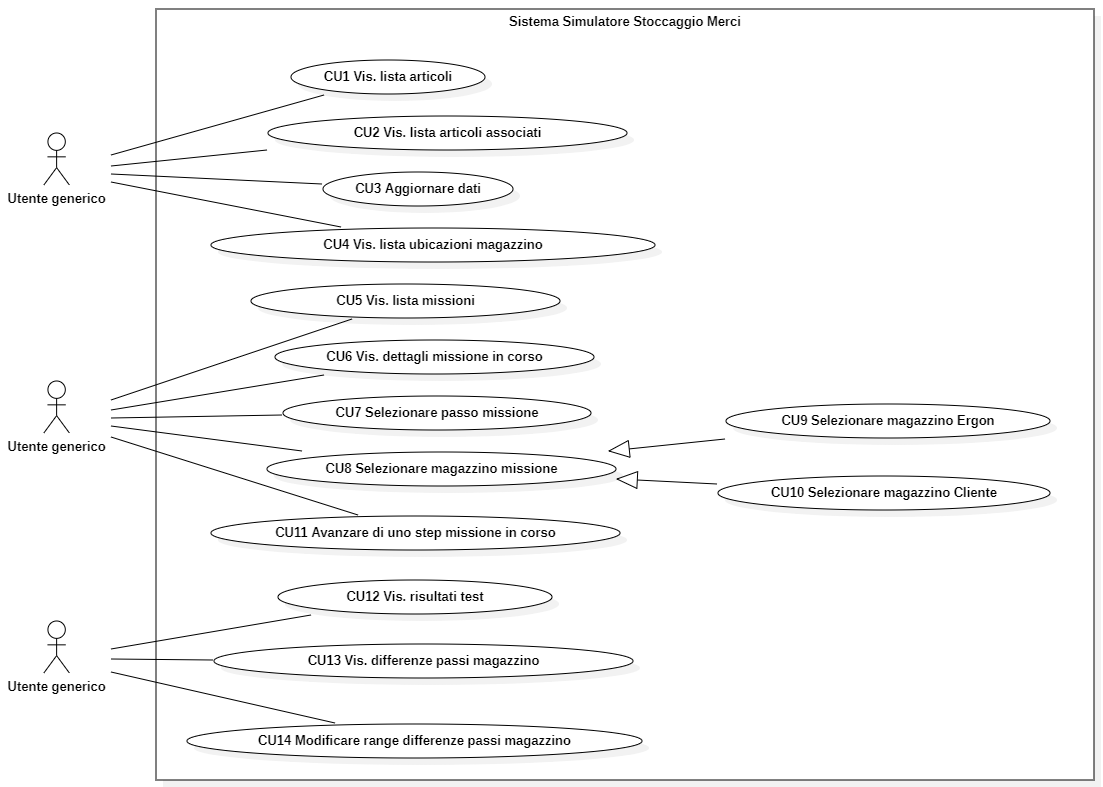
\includegraphics[width=1.5\columnwidth]{../images/usecase/generale} 
    }
    \caption{Casi d'uso - Sky level}
\end{figure}


\begin{usecase}{1}{Vis. lista articoli}
\usecaseactors{Utente generico}
\usecasepre{Nessuna}
\usecasedesc{La finestra mette a disposizione la visualizzazione della lista degli articoli con unità di misura "FS" che sono presenti in almeno un ordine cliente}
\usecasepost{L'utente visualizza la lista degli articoli con unità di misura "FS" che sono presenti in almeno un ordine cliente}
\textbf{\\Scenario Principale:}
\begin{itemize}
    \item L'utente apre la finestra per visualizzare la lista degli articoli.
\end{itemize}
\label{uc:scenario-principale}
\end{usecase}
%%%%%%%%%%%%%%%%%%%%%%%%%%%%%%%%%%%%%%%%%%%%%%%%%%%%%%
\begin{usecase}{2}{Vis. lista articoli associati}
    \usecaseactors{Utente generico}
    \usecasepre{Nessuna}
\usecasedesc{La finestra mette a disposizione la visualizzazione della lista degli articoli associati all'articolo selezionato nella lista articoli}
\usecasepost{L'utente visualizza la lista degli articoli associati all'articolo selezionato}
\textbf{\\Scenario Principale:}
\begin{itemize}
    \item L'utente apre la finestra per visualizzare la lista degli articoli;
    \item L'utente seleziona dalla lista articoli l'articolo di cui vuole visualizzare gli articoli associati.
\end{itemize}
\label{uc:scenario-principale}
\end{usecase}
%%%%%%%%%%%%%%%%%%%%%%%%%%%%%%%%%%%%%%%%%%%%%%%%%%%%%%
\begin{usecase}{3}{Aggiornare dati}
\usecaseactors{Utente generico}
\usecasepre{L'utente dispone delle autorizzazioni necessarie a interagire con il database}
\usecasedesc{L'utente aggiorna i dati relativi alla frequenza di vendita degli articoli e alla frequenza di associazione tra articoli presenti a database}
\textbf{\\Postcondizioni:}
\begin{itemize}
    \item I dati sulla frequenza di vendita e le associazioni degli articoli sono aggiornati a database.
\end{itemize}
\textbf{\\Scenario Principale:}
\begin{itemize}
    \item L'utente utilizza il comando "Aggiorna dati" per aggiornare i dati relativi alla frequenza di vendita e associazioni tra articoli presenti a database.
\end{itemize}
\label{uc:scenario-principale}
\end{usecase}
%%%%%%%%%%%%%%%%%%%%%%%%%%%%%%%%%%%%%%%%%%%%%%%%%%%%%%
\begin{usecase}{4}{Vis. lista ubicazioni magazzino}
\usecaseactors{Utente generico}
\usecasepre{L'utente ha avviato una simulazione di prelievo}
\usecasedesc{L'utente visualizza la disposizione degli articoli a magazzino}
\textbf{\\Postcondizioni:}
\begin{itemize}
    \item La disposizione degli articoli a magazzino è visibile.
\end{itemize}
\textbf{\\Scenario Principale:}
\begin{itemize}
    \item L'utente utilizza il comando "Avvia simulazione" per avviare una simulazione di prelievo.
\end{itemize}
\label{uc:scenario-principale}
\end{usecase}
%%%%%%%%%%%%%%%%%%%%%%%%%%%%%%%%%%%%%%%%%%%%%%%%%%%%%%
\begin{usecase}{5}{Vis. lista missioni}
\usecaseactors{Utente generico}
\usecasepre{L'utente ha avviato una simulazione di prelievo}
\usecasedesc{L'utente visualizza la missione di prelievo in corso e passate relative alla simulazione di prelievo}
\textbf{\\Postcondizioni:}
\begin{itemize}
    \item La missione di prelievo in corso è visibile;
    \item Le missioni di prelievo passate sono visibili.
\end{itemize}
\textbf{\\Scenario Principale:}
\begin{itemize}
    \item L'utente utilizza il comando "Avvia simulazione" per avviare una simulazione di prelievo.
\end{itemize}
\label{uc:scenario-principale}
\end{usecase}
%%%%%%%%%%%%%%%%%%%%%%%%%%%%%%%%%%%%%%%%%%%%%%%%%%%%%%
\begin{usecase}{6}{Vis. dettagli missione in corso}
\usecaseactors{Utente generico}
\usecasepre{L'utente ha avviato una simulazione di prelievo}
\usecasedesc{L'utente visualizza lo stato della missione in corso}
\textbf{\\Postcondizioni:}
\begin{itemize}
    \item Lo stato della missione in corso è visibile.
\end{itemize}
\textbf{\\Scenario Principale:}
\begin{itemize}
    \item L'utente utilizza il comando "Avvia simulazione" per avviare una simulazione di prelievo.
\end{itemize}
\label{uc:scenario-principale}
\end{usecase}
%%%%%%%%%%%%%%%%%%%%%%%%%%%%%%%%%%%%%%%%%%%%%%%%%%%%%%
\begin{usecase}{7}{Selezionare passo missione}
\usecaseactors{Utente generico}
\usecasepre{L'utente ha avviato una simulazione di prelievo}
\usecasedesc{L'utente modifica il passo associazioni con cui vengono disposti gli articoli a magazzino}
\textbf{\\Postcondizioni:}
\begin{itemize}
    \item La simulazione di prelievo è ripristinata allo stato iniziale;
    \item La disposizione degli articoli a magazzino è aggiornata secondo il passo selezionato dall'utente.
\end{itemize}
\textbf{\\Scenario Principale:}
\begin{itemize}
    \item L'utente modifica il passo missione utilizzando la form dedicata.
\end{itemize}
\label{uc:scenario-principale}
\end{usecase}
%%%%%%%%%%%%%%%%%%%%%%%%%%%%%%%%%%%%%%%%%%%%%%%%%%%%%%
\begin{usecase}{8}{Selezionare magazzino missione}
    \textbf{\\Generalizzazione di:}
\begin{itemize}
    \item CU9 Selezionare magazzino Ergon;
    \item CU10 Selezionare magazzino cliente.
\end{itemize}
\usecaseactors{Utente generico}
\usecasepre{L'utente ha avviato una simulazione di prelievo}
\usecasedesc{L'utente seleziona il magazzino sul quale effettuare la simulazione}
\textbf{\\Postcondizioni:}
\begin{itemize}
    \item La simulazione di prelievo è ripristinata allo stato iniziale;
    \item La disposizione degli articoli a magazzino è aggiornata secondo il magazzino selezionato dall'utente.
\end{itemize}
\textbf{\\Scenario Principale:}
\begin{itemize}
    \item L'utente seleziona il magazzino sul quale effettuare la missione utilizzando la form dedicata.
\end{itemize}
\label{uc:scenario-principale}
\end{usecase}
%%%%%%%%%%%%%%%%%%%%%%%%%%%%%%%%%%%%%%%%%%%%%%%%%%%%%%
\begin{usecase}{9}{Selezionare magazzino Ergon}
\usecaseactors{Utente generico}
\usecasepre{L'utente ha avviato una simulazione di prelievo}
\usecasedesc{L'utente seleziona il magazzino Ergon sul quale effettuare la simulazione. Il magazzino Ergon è caratterizzato da una disposizione degli articoli che segue il passo associazione
articoli selezionato dall'utente}
\textbf{\\Postcondizioni:}
\begin{itemize}
    \item La simulazione di prelievo è ripristinata allo stato iniziale;
    \item La disposizione degli articoli a magazzino è aggiornata secondo il magazzino Ergon rispettando il passo selezionato dall'utente;
    \item La funzionalità di selezione passo magazzino è abilitata.
\end{itemize}
\textbf{\\Scenario Principale:}
\begin{itemize}
    \item L'utente seleziona il magazzino Ergon sul quale effettuare la missione utilizzando la form dedicata.
\end{itemize}
\label{uc:scenario-principale}
\end{usecase}
%%%%%%%%%%%%%%%%%%%%%%%%%%%%%%%%%%%%%%%%%%%%%%%%%%%%%%
\begin{usecase}{10}{Selezionare magazzino cliente}
\usecaseactors{Utente generico}
\usecasepre{L'utente ha avviato una simulazione di prelievo}
\usecasedesc{L'utente seleziona il magazzino cliente sul quale effettuare la simulazione. Il magazzino cliente rispetta fedelmente la disposizione attuale del magazzino cliente e non applica un passo 
associazione prodotti}
\textbf{\\Postcondizioni:}
\begin{itemize}
    \item La simulazione di prelievo è ripristinata allo stato iniziale;
    \item La disposizione degli articoli a magazzino è aggiornata secondo il magazzino cliente;
    \item La funzionalità di selezione passo magazzino è disabilitata.
\end{itemize}
\textbf{\\Scenario Principale:}
\begin{itemize}
    \item L'utente seleziona il magazzino cliente sul quale effettuare la missione utilizzando la form dedicata.
\end{itemize}
\label{uc:scenario-principale}
\end{usecase}
%%%%%%%%%%%%%%%%%%%%%%%%%%%%%%%%%%%%%%%%%%%%%%%%%%%%%%
\begin{usecase}{11}{Avanzare di uno step missione in corso}
\usecaseactors{Utente generico}
\textbf{\\Precondizioni:}
\begin{itemize}
    \item Nella simulazionie di prelievo è presente almeno una missione non terminata;
    \item La missione attuale si trova ad uno step di partenza.
\end{itemize}
\usecasedesc{L'utente avanza di uno step nella missione in corso. Avanzare di uno step permette di visualizzare lo stato del carrello alla fermata successiva rispetto allo step missione attuale}
\textbf{\\Postcondizioni:}
\begin{itemize}
    \item La missione attuale si trova allo step successivo allo step di partenza.
\end{itemize}
\textbf{\\Scenario Principale:}
\begin{itemize}
    \item L'utente utilizza il comando "Avanza step missione" per avanzare di uno step missione.
\end{itemize}
\label{uc:scenario-principale}
\end{usecase}
%%%%%%%%%%%%%%%%%%%%%%%%%%%%%%%%%%%%%%%%%%%%%%%%%%%%%%
\begin{usecase}{12}{Vis. risultati test}
\usecaseactors{Utente generico}
\usecasepre{Nessuna}
\usecasedesc{L'utente visualizza i risultati della simulazione effettuata sul magazzino cliente e di tutte le simulazioni effettuate sul magazzino Ergon a tutti i passi previsti dal sistema di 
simulazione}
\usecasepost{I risultati di tutte le simulazioni effettuate sono visibili all'utente}
\textbf{\\Scenario Principale:}
\begin{itemize}
    \item L'utente utilizza il comando "Visualizza risultati test" per visualizzare i risultati dei test.
\end{itemize}
\label{uc:scenario-principale}
\end{usecase}
%%%%%%%%%%%%%%%%%%%%%%%%%%%%%%%%%%%%%%%%%%%%%%%%%%%%%%
\begin{usecase}{13}{Vis. differenze passi magazzino}
\usecaseactors{Utente generico}
\usecasepre{Nessuna}
\usecasedesc{L'utente visualizza le differenze tra le diverse configurazioni di magazzino Ergon che dipendono dai passi associazioni.Le differenze vengono visualizzate tenendo conto 
del range di ubicazioni selezionate dell'utente entro il quale si vogliono visualizzare le differenze tra le configurazioni di magazzino}
\usecasepost{Le differenze tra le diverse configurazioni di magazzino Ergon sono visibili all'utente}
\textbf{\\Scenario Principale:}
\begin{itemize}
    \item L'utente utilizza il comando "Visualizza differenze passi" per visualizzare le differenze tra le diverse configurazioni di magazzino Ergon.
\end{itemize}
\label{uc:scenario-principale}
\end{usecase}
%%%%%%%%%%%%%%%%%%%%%%%%%%%%%%%%%%%%%%%%%%%%%%%%%%%%%%
\begin{usecase}{14}{Modificare range differenze passi magazzino}
\usecaseactors{Utente generico}
\usecasepre{L'utente visualizza le differenze passi magazzino in un range di partenza}
\usecasedesc{L'utente modifica il range differenze passi magazzino per visualizzare le differenze tra le diverse configurazioni di magazzino in un range diverso da quello di partenza}
\textbf{\\Postcondizioni:}
\begin{itemize}
    \item Il range di visualizzazione differenze passi magazzino è stato modificato;
    \item Le differenze tra le configurazioni di magazzino sono state aggiornate secondo il range impostato;
    \item Le differenze tra le diverse configurazioni di magazzino Ergon sono visibili all'utente.
\end{itemize}
\textbf{\\Scenario Principale:}
\begin{itemize}
    \item L'utente utilizza il comando "Modifica range" per aggiornare la visualizzazione delle differenze tra le diverse configurazioni di magazzino Ergon.
\end{itemize}
\label{uc:scenario-principale}
\end{usecase} 
%%%%%%%%%%%%%%%%%%%%%%%%%%%%%%%%%%%%%%%%%%%%%%%%%%%%%%
\begin{figure}[!h] 
    \centering 
    \makebox[\textwidth]{
    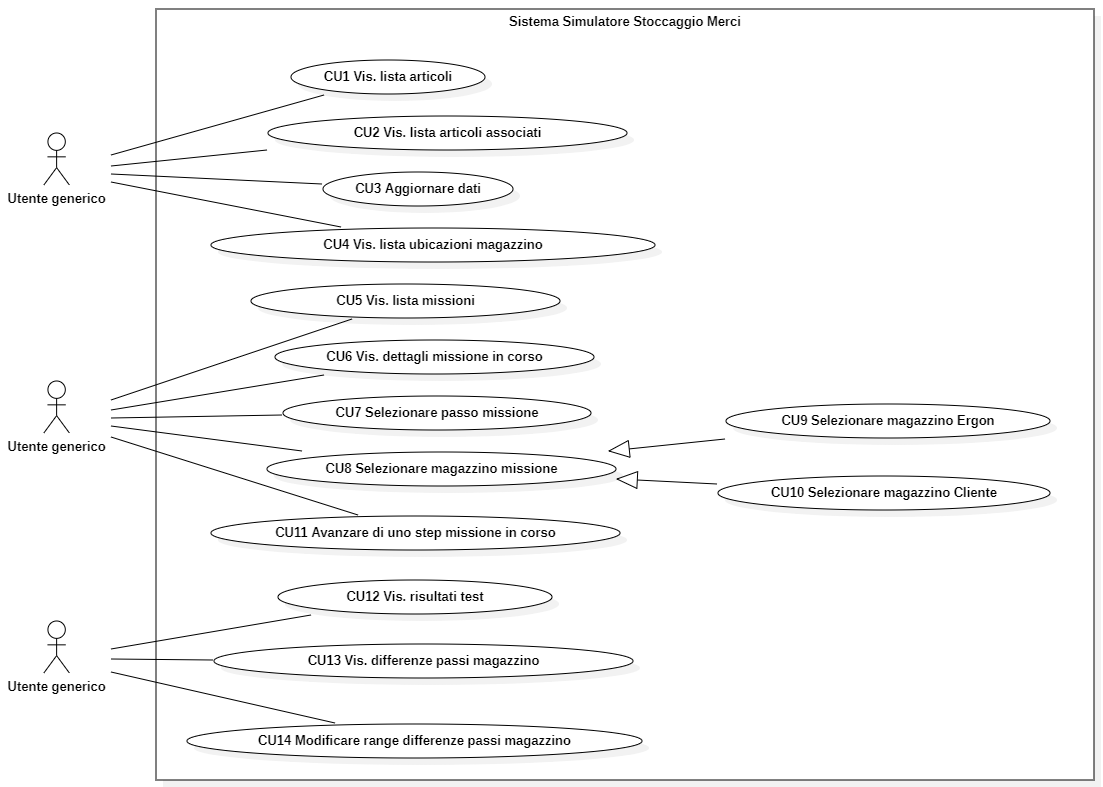
\includegraphics[width=1.5\columnwidth]{../images/usecase/generale} 
    }
    \caption{Casi d'uso - Sky level}
\end{figure}







% \section{Tracciamento dei requisiti}

% Da un'attenta analisi dei requisiti e degli use case effettuata sul progetto è stata stilata la tabella che traccia i requisiti in rapporto agli use case.\\
% Sono stati individuati diversi tipi di requisiti e si è quindi fatto utilizzo di un codice identificativo per distinguerli.\\
% Il codice dei requisiti è così strutturato R(F/Q/V)(N/D/O) dove:
% \begin{enumerate}
% 	\item[R =] requisito
%     \item[F =] funzionale
%     \item[Q =] qualitativo
%     \item[V =] di vincolo
%     \item[N =] obbligatorio (necessario)
%     \item[D =] desiderabile
%     \item[Z =] opzionale
% \end{enumerate}
% Nelle tabelle \ref{tab:requisiti-funzionali}, \ref{tab:requisiti-qualitativi} e \ref{tab:requisiti-vincolo} sono riassunti i requisiti e il loro tracciamento con gli use case delineati in fase di analisi.

% \newpage

% \begin{table}%
% \caption{Tabella del tracciamento dei requisti funzionali}
% \label{tab:requisiti-funzionali}
% \begin{tabularx}{\textwidth}{lXl}
% \hline\hline
% \textbf{Requisito} & \textbf{Descrizione} & \textbf{Use Case}\\
% \hline
% RFN-1     & L'interfaccia permette di configurare il tipo di sonde del test & UC1 \\
% \hline
% \end{tabularx}
% \end{table}%

% \begin{table}%
% \caption{Tabella del tracciamento dei requisiti qualitativi}
% \label{tab:requisiti-qualitativi}
% \begin{tabularx}{\textwidth}{lXl}
% \hline\hline
% \textbf{Requisito} & \textbf{Descrizione} & \textbf{Use Case}\\
% \hline
% RQD-1    & Le prestazioni del simulatore hardware deve garantire la giusta esecuzione dei test e non la generazione di falsi negativi & - \\
% \hline
% \end{tabularx}
% \end{table}%

% \begin{table}%
% \caption{Tabella del tracciamento dei requisiti di vincolo}
% \label{tab:requisiti-vincolo}
% \begin{tabularx}{\textwidth}{lXl}
% \hline\hline
% \textbf{Requisito} & \textbf{Descrizione} & \textbf{Use Case}\\
% \hline
% RVO-1    & La libreria per l'esecuzione dei test automatici deve essere riutilizzabile & - \\
% \hline
% \end{tabularx}
% \end{table}%
